% CryptAgent BTP-III: implementation and observed results.
% Edit the three names and contribution statements before presenting.
\documentclass[aspectratio=169,10pt]{beamer}
\usetheme{Madrid}
\usecolortheme{default}
\usepackage[T1]{fontenc}
\usepackage{lmodern}
\usepackage{booktabs}
\usepackage{tabularx}
\usepackage{array}
\usepackage{tikz}
\usetikzlibrary{arrows.meta,positioning}
\definecolor{cryptblue}{HTML}{173B70}
\definecolor{cryptteal}{HTML}{0B7A78}
\setbeamercolor{structure}{fg=cryptblue}
\setbeamercolor{frametitle}{fg=white,bg=cryptblue}
\setbeamercolor{block title}{fg=white,bg=cryptteal}
\setbeamertemplate{navigation symbols}{}
\setbeamertemplate{footline}[frame number]
\newcommand{\mone}{Member 1 (name)}
\newcommand{\mtwo}{Member 2 (name)}
\newcommand{\mthree}{Member 3 (name)}
\title[CryptAgent: BTP-III]{CryptAgent\\Implementation and observed results}
\subtitle{BTP-III: AES-only local source-review prototype}
\author[Three-member team]{\mone\\[0.2em]\mtwo\\[0.2em]\mthree}
\institute{Three-member BTP project team}
\date{\today}

\begin{document}
\begin{frame}\titlepage\end{frame}

\begin{frame}{What was implemented}
\begin{itemize}
\item A browser interface for one fixed profile: AES-128-GCM, C++20, Windows CNG, message tampering.
\item A Node.js backend with input validation, source observations, strict model-output checking and JSON reports.
\item A local Python service running cached Llama-3.1-8B-Instruct on the laboratory GPU.
\item An AES dataset \emph{candidate}: 22 train, four validation and four test examples.
\end{itemize}
\begin{alertblock}{Current evidence level}
The pipeline performs advisory source review. Submitted C++ is not compiled or executed by this web app.
\end{alertblock}
\end{frame}

\begin{frame}{Implementation architecture}
\centering
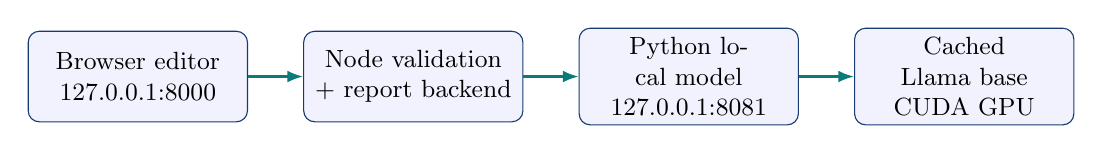
\begin{tikzpicture}[node distance=0.55cm and 0.7cm, every node/.style={font=\small},
 box/.style={draw=cryptblue,rounded corners,fill=blue!5,text width=2.55cm,minimum height=1.15cm,align=center},
 arr/.style={-{Latex[length=2mm]},thick,draw=cryptteal}]
\node[box] (web) {Browser editor\\127.0.0.1:8000};
\node[box,right=of web] (node) {Node validation + report backend};
\node[box,right=of node] (py) {Python local model\\127.0.0.1:8081};
\node[box,right=of py] (gpu) {Cached Llama base\\CUDA GPU};
\draw[arr] (web)--(node); \draw[arr] (node)--(py); \draw[arr] (py)--(gpu);
\end{tikzpicture}
\vspace{1em}
\begin{itemize}
\item The model endpoint is fixed to loopback; there is no external API key or remote source-code call.
\item The local service reports loading, ready, busy and error states.
\end{itemize}
\end{frame}

\begin{frame}{Frontend and backend responsibilities}
\small
\begin{tabularx}{\textwidth}{>{\bfseries}p{3.1cm}X}
\toprule
Component & Implemented behavior \\
\midrule
Frontend & Paste/open C++ source; show line numbers, model status, five checks, linked findings and JSON export. \\
\texttt{app.mjs} & Serve UI; validate host/origin, token, profile and input bounds; allow one active review. \\
\texttt{verifier.mjs} & Record source-pattern observations and assemble advisory report. \\
\texttt{llm\_client.mjs} & Call local model; check service identity, prompt hash, time and response size. \\
\texttt{review\_contract.mjs} & Validate exact JSON keys, five F01--F05 IDs and quoted source lines. \\
\bottomrule
\end{tabularx}
\end{frame}

\begin{frame}{The code-review workflow}
\begin{enumerate}
\item Browser obtains the fixed profile and session token from \texttt{GET /api/status}.
\item User submits code to \texttt{POST /api/verify}; Node checks input and hashes source.
\item Node sends source to local \texttt{POST /review}; Python creates a line-numbered prompt and runs Llama.
\item Node validates the returned five-check JSON and exact source quotations.
\item Node combines model findings and separately labeled source observations; browser displays/export the report.
\end{enumerate}
\vspace{0.4em}
\alert{Model interpretation is advisory even when the JSON and source quotation are valid.}
\end{frame}

\begin{frame}{Active model configuration}
\begin{itemize}
\item Cached \texttt{meta-llama/Llama-3.1-8B-Instruct} base model; pinned revision, offline loading.
\item PyTorch + Transformers + bitsandbytes; 4-bit weights on CUDA with bfloat16 computation.
\item Deterministic generation configuration; maximum 3,072 input tokens and bounded output/time.
\item A prompt specifies the fixed AES/CNG profile and source-linked JSON answer.
\item An experimental AES adapter was trained, but not activated for this web service.
\end{itemize}
\begin{block}{Privacy boundary}
Submitted code travels between two services on the same machine, bound to \texttt{127.0.0.1}. Neither service saves the submitted source in the normal review path.
\end{block}
\end{frame}

\begin{frame}{Outputs and failure behavior}
\small
\begin{tabularx}{\textwidth}{>{\ttfamily}p{4.2cm}X}
\toprule
Verdict & Meaning \\
\midrule
potential\_issues & At least one model finding or source observation needs review. \\
no\_issues\_identified & No issue found in visible source; not a security proof. \\
insufficient\_context & The relevant implementation or lifecycle is missing. \\
outside\_scope & The model classified the code outside fixed AES/CNG scope. \\
review\_unavailable & The model was offline, incomplete or invalid; no model conclusion accepted. \\
\bottomrule
\end{tabularx}
\vspace{0.7em}
Invalid input and timeouts are explicit. The report marks native execution and formal verification \texttt{not\_run}.
\end{frame}

\begin{frame}{Validation results: what passed}
\begin{columns}[T]
\column{0.45\textwidth}
\begin{block}{Automated contracts}
11 Node tests and four Python HTTP tests passed: routing, input guards, JSON consistency, source quotations and failure paths.
\end{block}
\column{0.53\textwidth}
\begin{block}{Real GPU smoke tests}
Three synthetic submissions produced reports: unrelated Python \(\rightarrow\) outside scope; declarations \(\rightarrow\) insufficient context; discarded decrypt status \(\rightarrow\) potential issues.
\end{block}
\end{columns}
\vspace{0.8em}
\centering\alert{These measure pipeline operation, not cryptographic detection accuracy.}
\end{frame}

\begin{frame}{Observed model errors and analysis}
\begin{itemize}
\item In the ignored-status example, the source-pattern scanner found the concern, but the base model marked the individual F03 check too optimistically.
\item In incomplete examples, the base model sometimes marked requirements as having no issue despite missing context.
\item Stronger prompt wording was tried; it regressed on example outputs and was reverted.
\end{itemize}
\begin{alertblock}{Interpretation}
A formatted and source-linked answer can still contain an incorrect security judgment. This motivates independent labels, abstention checks and held-out evaluation.
\end{alertblock}
\end{frame}

\begin{frame}{Dataset work and training status}
\small
\begin{tabularx}{\textwidth}{>{\bfseries}p{3.6cm}X}
\toprule
Split & Current AES candidate \\
\midrule
Training & 22 unique codes: 16 short snippets and six related full-session variants. \\
Validation & Four historical AES development examples. \\
Test & Four historical AES development examples. \\
Total & 30 normalized-unique code samples; longest prompt/answer sequence: 3,049 tokens. \\
\bottomrule
\end{tabularx}
\vspace{0.7em}
\begin{itemize}
\item Fixed F01--F05 labels and source quotations pass the production response validator.
\item Full-session label review and a fresh independent evaluation split are pending.
\item An experimental two-epoch adapter was trained from 22 rows; the manifest remains \texttt{training\_ready=false}.
\item Its 20-case source-only comparison is exploratory, not independent security validation.
\end{itemize}
\end{frame}

\begin{frame}{Exploratory AES adapter comparison}
\small
\begin{tabularx}{\textwidth}{>{\bfseries}p{5.0cm}XX}
\toprule
Metric on 20 new synthetic excerpts & Base & Adapter \\
\midrule
Fully accepted output & 7/20 & 20/20 \\
Correctly located target concern & 0/13 & 3/13 \\
Safe controls without a false alarm & 3/4 & 3/4 \\
Correct scope & 17/20 & 19/20 \\
\bottomrule
\end{tabularx}
\vspace{0.7em}
\alert{Formatting improved more than defect detection. The adapter is not approved for deployment.}
\end{frame}

\begin{frame}{Expansion research is separate from the active app}
\begin{itemize}
\item Python/TenSEAL CKKS, Rust/TFHE-rs and C++/OpenFHE BFV fixtures explore distinct key, result and input boundaries.
\item Authored faulty/corrected pairs and native probes are retained as research evidence.
\item FHE-specific H01--H05 requirements are not interchangeable with AES F01--F05.
\item The web application remains AES-only; selectable profiles and generation are future work.
\end{itemize}
\end{frame}

\begin{frame}{Historical results are kept separate}
\begin{itemize}
\item Phase 1--3 preserved a different libsodium/XChaCha20-Poly1305 contract with 13 requirements.
\item The historical synthetic benchmark contains 150 cases from 30 related scenario groups, not 150 independent codebases.
\item Older package/schema checks and a syntax-only Windows C++ header test are documented; native candidate execution was not completed in that historical validation.
\item These do not establish current AES/Windows CNG runtime correctness.
\end{itemize}
\end{frame}

\begin{frame}{Current limitations and next measurements}
\begin{columns}[T]
\column{0.48\textwidth}
\textbf{Present limits}
\begin{itemize}
\item No native Windows CNG tests for submitted code.
\item Base model active; experimental adapter has a small synthetic comparison, not an independent accuracy result.
\item Pattern matches are observations, not confirmed vulnerabilities.
\end{itemize}
\column{0.50\textwidth}
\textbf{Next evaluation}
\begin{itemize}
\item Review labels and collect fresh implementation families.
\item Record defect recall, false positives, abstention and cited-line accuracy.
\item Improve reviewed labels and compare a revised adapter against the base on a fresh frozen test.
\end{itemize}
\end{columns}
\end{frame}

\begin{frame}{Live demonstration plan}
\begin{enumerate}
\item Start \texttt{bash start.sh}; open \texttt{http://127.0.0.1:8000}.
\item Show the fixed AES-128-GCM/C++20/CNG/message-tampering profile.
\item Submit a small decryption excerpt that discards \texttt{BCryptDecrypt} status.
\item Show a cited source line, five assessments and JSON export.
\item Submit unrelated or incomplete code; show outside-scope/needs-context handling.
\item Point out \texttt{candidateExecuted=false} and \texttt{not\_run} native checks.
\end{enumerate}
\end{frame}

\begin{frame}{Three members: individual implementation contributions}
\small
\begin{tabularx}{\textwidth}{>{\bfseries}p{2.7cm}X}
\toprule
Team member & Replace with the member's \emph{actual} BTP-III contribution \\
\midrule
\mone & Frontend, interaction or demo work: \textbf{[edit to actual files and validation]}. \\
\mtwo & Backend, profile, report contract or security boundary: \textbf{[edit to actual files and validation]}. \\
\mthree & Local model, dataset audit or test work: \textbf{[edit to actual files and validation]}. \\
\bottomrule
\end{tabularx}
\vspace{0.6em}
{\scriptsize These are placeholders only. Give each member a separate spoken explanation of specific work and evidence.}
\end{frame}

\begin{frame}{Conclusion}
\begin{block}{Implemented result}
The fixed-profile, local AES source-review pipeline runs end to end and returns source-linked, explicitly limited reports.
\end{block}
\begin{block}{Evidence still required}
Independent accuracy evaluation, reviewed AES labels, an activated fine-tuned model and native Windows CNG witnesses remain future work.
\end{block}
\end{frame}

\begin{frame}{References and reproducibility}
\scriptsize
\begin{thebibliography}{9}
\bibitem{nist} NIST, \emph{SP 800-38D: GCM and GMAC}. \url{https://csrc.nist.gov/pubs/sp/800/38/d/final}
\bibitem{dec} Microsoft, \emph{BCryptDecrypt function}. \url{https://learn.microsoft.com/en-us/windows/win32/api/bcrypt/nf-bcrypt-bcryptdecrypt}
\bibitem{repo} CryptAgent local repository: \texttt{README.md}, \texttt{STATUS.md}, \texttt{docs/AES\_REVIEW\_CONTRACT.md}, \texttt{tests/}, and \texttt{training/aes\_source\_pilot\_v1/data/manifest.json}.
\end{thebibliography}
\end{frame}
\end{document}
